\PassOptionsToPackage{top=3cm,left=3cm,right=3cm,bottom=3cm}{geometry}
\documentclass[fleqn,11pt]{wlscirep_supp}

\usepackage[]{minitoc}
\mtcsetdepth{secttoc}{3}
\setcounter{secnumdepth}{2}
\setcounter{tocdepth}{2}
\mtcsettitle{secttoc}{}


\usepackage[utf8]{inputenc}
\usepackage[T1]{fontenc}
\usepackage[english]{babel}
%\usepackage[top=3cm,left=3cm,right=3cm,bottom=3cm]{geometry}% by courtesy of Mico
\usepackage{lmodern}
\usepackage{bbm}
\usepackage{graphicx}
\usepackage{epstopdf}
\usepackage{colortbl}
\usepackage{siunitx}
\sisetup{
  detect-all,
  detect-weight=true,
  detect-family=true,
  mode=text,
%   detect-inline-family=math,
  group-separator={,},
%   group-minimum-digits={3}			
}
\usepackage{rotating}
\usepackage{tabularx}
\usepackage{tabu}
\usepackage{authblk}
\usepackage{mathtools}
\usepackage{overpic}
\usepackage{url}
\usepackage{tikz}
\usetikzlibrary{positioning}
\usetikzlibrary{arrows}
\usetikzlibrary{fit}
\usepackage{multirow}
\usepackage{float}
\usepackage[normalem]{ulem}
\usepackage{bm}
\usepackage{enumerate}
\usepackage[absolute,overlay%,showboxes
                        ]{textpos}
% \usepackage{caption}
\usepackage[font=small,labelfont=bf,justification=justified]{caption}
\usepackage{subcaption}
\usepackage{xspace}
\usepackage[colorinlistoftodos]{todonotes}
\usepackage{placeins}
\usepackage{makecell, booktabs}
\usepackage{eqparbox}
\usepackage{rotating}
\usepackage{graphicx}
\usepackage{xspace}
\usepackage{setspace}
%\usepackage{comment}
\usepackage[resetlabels,labeled]{multibib}
\newcites{Supp}{References}
\usepackage[sort&compress]{cleveref}
\Crefname{appendix}{Supplement}{Supplements}

%\usepackage{mathabx}

% Table formatting packages
\usepackage{dcolumn} % align decimal points in tables
\newcolumntype{d}[1]{D{.}{.}{#1}}
\usepackage{booktabs} 
\usepackage[flushleft]{threeparttable}
\usepackage{siunitx} % align on decimal point in tables
\usepackage{lineno}
\usepackage{etoolbox}

\usepackage{lscape}
\usepackage{longtable}
\usepackage{arydshln}

% math
\usepackage{amsmath,amsfonts,amssymb}
% additional math symbols
\DeclareFontFamily{U}{mathb}{}
\DeclareFontShape{U}{mathb}{m}{n}{
  <-5.5> mathb5
  <5.5-6.5> mathb6
  <6.5-7.5> mathb7
  <7.5-8.5> mathb8
  <8.5-9.5> mathb9
  <9.5-11.5> mathb10
  <11.5-> mathb12
}{}
\DeclareSymbolFont{mathb}{U}{mathb}{m}{n}
\DeclareMathSymbol{\ulsh}{3}{mathb}{"E8}
\DeclareMathSymbol{\ursh}{3}{mathb}{"E9}
\DeclareMathSymbol{\dlsh}{3}{mathb}{"EA}
\DeclareMathSymbol{\drsh}{3}{mathb}{"EB}

%% Patch 'normal' math environments:
\newcommand*\linenomathpatch[1]{%
  \cspreto{#1}{\linenomath}%
  \cspreto{#1*}{\linenomath}%
  \csappto{end#1}{\endlinenomath}%
  \csappto{end#1*}{\endlinenomath}%
}

\linenomathpatch{equation}
\linenomathpatch{gather}
\linenomathpatch{multline}
\linenomathpatch{align}
\linenomathpatch{alignat}
\linenomathpatch{flalign}

\linenumbers

% PLOS formatting
\makeatletter %only needed in preamble
\renewcommand\Large{\@setfontsize\Large{18pt}{18}}
\renewcommand\large{\@setfontsize\large{16pt}{18}}
\makeatother

\addto\captionsenglish{\renewcommand{\figurename}{Figure}}

% \usepackage{xstring}
% \usepackage{etoolbox}
% \usepackage{caption}

% \captionsetup{labelfont=bf,tableposition=top}

% \makeatletter
% \newcommand\formatlabel[1]{%
%     \noexpandarg
%     \IfSubStr{#1}{.}{%
%       \StrBefore{#1}{.}[\firstcaption]%
%       \StrBehind{#1}{.}[\secondcaption]%
%       \textbf{\firstcaption.} \secondcaption}{%
%       #1}%
%       }


% \patchcmd{\@caption}{#3}{\formatlabel{#3}}
% \makeatother

\renewcommand*{\Affilfont}{\normalsize\normalfont}
\renewcommand*{\Authfont}{\normalfont}


% referencing of unnumbered materials and methods
\newcounter{methods}
\renewcommand{\themethods}{Materials and methods}

% Track changes
%\usepackage[markup=underlined]{changes}
\makeatletter
\@namedef{Changes@AuthorColor}{magenta}
\colorlet{Changes@Color}{magenta}
\makeatother


%=====================================================================% Declare

\DeclareSIUnit\eur{\officialeuro}
\DeclareSIUnit\M{M}
\DeclareSIUnit\k{k}

% Widebar symbol
% \DeclareFontFamily{U}{mathx}{\hyphenchar\font45}
% \DeclareFontShape{U}{mathx}{m}{n}{<-> mathx10}{}
% \DeclareSymbolFont{mathx}{U}{mathx}{m}{n}
% \DeclareMathAccent{\widebar}{0}{mathx}{"73}

%=====================================================================% New commands (Macros)

% def
\def\sym#1{\ifmmode^{#1}\else\(^{#1}\)\fi}
\definecolor{darkgreen}{rgb}{0.0, 0.5, 0.0}

% new command
\newcommand{\smallsim}{\smallsym{\mathrel}{\sim}}
\newcommand{\specialcell}[2][c]{%
  \begin{tabular}[#1]{@{}l@{}}#2\end{tabular}}
\newcommand{\specialcellc}[2][c]{%
  \begin{tabular}[#1]{@{}c@{}}#2\end{tabular}}
\newcommand\ie{i.\,e.\xspace}
\newcommand\eg{e.\,g.\xspace}
\newcommand{\dd}[1][]{\mathrm{d}#1}
\newcommand{\BK}[1]{{\color{orange}{BK: #1}}}
\newcommand{\figletter}[1]{{{\fontfamily{\sfdefault}\selectfont \textbf{#1}}}}
\newcommand\TODO[1]{{\color{red}#1}}  
\newcommand{\FIX}[1]{{\color{darkgreen}#1}}  

% renewcommand
\renewcommand\theadfont{\bfseries}
\renewcommand\theadalign{lc}
\renewcommand\cellalign{tl}

\makeatletter

\newbox\@abstract%
\def\abstitle{\textbf{Abstract}}%
\renewenvironment{abstract}{
  \global\setbox\@abstract\vbox\bgroup%
   \noindent
}{%
   \egroup%
}%

\renewcommand*{\Affilfont}{\normalsize\normalfont}
\renewcommand*{\Authfont}{\normalfont}

\addto\captionsenglish{% Replace "english" with the language you use
  \renewcommand{\contentsname}{List of Texts}
}

\def\@maketitle{%
  \newpage
    {\raggedright\fontsize{18pt}{20pt}\selectfont \@title \par}%
    \vskip 0.5em%
    {\large
      \lineskip .5em%
      \begin{tabular}[t]{l}%
        \raggedright \normalsize\mdseries{\@author} %
      \end{tabular}\par}%
      \vskip 1em
%      \raggedright\Large\abstitle\par
%      \vskip 1em
%    {\unvbox\@abstract\par}%
    \par
  \vskip 0.5em
}
  
\makeatother


\renewcommand{\thesection}{Text \arabic{section}}
\usepackage{titlesec}
%\titleformat{\section}{\normalfont\Large\bfseries}{Text \thesection.~#1}{1em}{}
\renewcommand{\thefigure}{S\arabic{figure}}
\renewcommand{\thetable}{S\arabic{table}}

\begin{document}
\doublespacing
\nolinenumbers

\newcommand{\supp}{SI Appendix}

\title{\LARGE\singlespacing{\textbf{Supplementary Material} \\ \medskip
Molecular detection of SARS-CoV-2 and other respiratory viruses in saliva and classroom air: a two winters tale}}

% long: Air cleaners and respiratory infections in schools: \\ A modeling study using epidemiological, environmental, and molecular data

% author list
% author list
\author[1,2]{Nicolas Banholzer}
\author[2,4]{Pascal Bittel}
\author[2,3]{Philipp Jent}
\author[4]{Lavinia Furrer}
\author[1]{Kathrin Zürcher}
%\author[1]{Simon Bertschinger}
%\author[5]{Ernest Weingartner}
%\author[2,4]{Alban Ramette}
\author[1,6,7]{Matthias Egger}
\author[2,8]{Tina Hascher}
\author[1*,2]{Lukas Fenner}

\affil[1]{Institute of Social and Preventive Medicine, University of Bern, Bern, Switzerland}
\affil[2]{Multidisciplinary Center for Infectious Diseases, University of Bern, Bern, Switzerland}
\affil[3]{Department of Infectious Diseases, Inselspital, Bern University Hospital, University of Bern, Bern, Switzerland}
\affil[4]{Institute for Infectious Diseases, University of Bern, Bern, Switzerland}
%\affil[5]{Institute for Sensors and Electronics, University of Applied Sciences and Arts Northwestern Switzerland, Windisch, Switzerland}
\affil[5]{Population Health Sciences, University of Bristol, Bristol, UK}
\affil[6]{Centre for Infectious Disease Epidemiology and Research, University of Cape Town, Cape Town, South Africa}
\affil[7]{Institute of Educational Science, University of Bern, Bern, Switzerland}

%\begin{abstract}\normalfont
%The supplementary material contains (1)~the detailed method, (2)~the simulation-based study, (3)~further descriptives, and (4)~the results from the sensitivity analysis.
%\end{abstract}

\flushbottom
\maketitle
\thispagestyle{empty}

%\newpage

\sloppy
\raggedbottom

\newpage

\appendix

\begin{table}[!htpb]
    \caption{Comparison of the study settings in winter 2021/22 and 2022/23.}
    \label{tab:comp_study}
    \centering
    \renewcommand{\arraystretch}{1.5}
    \begin{tabular}{lp{6cm}p{6cm}}
        \toprule
        & \textbf{Winter 2021/22} & \textbf{Winter 2022/23} \\
        \midrule
        Participants & two classes from School~1 sharing one classroom (half-class teaching) and one class from School~2 with a separate classroom; one teacher per lesson per classroom & two classes from School~2 with two separate classrooms (none of the two classes had already participated in winter 2021/23); one teacher per lesson per classroom \\
        Setting & School~1 and~2 are in different towns, which have grown together over the years and are situated in a urban/peri-urban environment & School 2 is the same as in the previous winter \\
        Duration & seven weeks per class (January 16 to March 11, 2023), excluding vacation & seven weeks per class (January 24 to March 26, 2023), excluding vacation \\
        Saliva testing & weekly (Wednesdays) & bi-weekly (Tuesdays and Thursdays) \\
        Bioaerosol sampling & daily with BioSpot-VIVAS and Coriolis in both classrooms & daily with BioSpot-VIVAS and Coriolis in one classroom and only Coriolis in the other classroom \\
        HEPA-filters samples & collected once at the end of the study & collected twice after the phases where the air cleaner intervention was in place \\
        Interventions & compulsory face mask wearing as mandated by the public health authorities at that time from the start of the study, for a total of six out of 14 study weeks; and installation of portable air cleaners towards the end of the study in the study classrooms for a total of four out of 14 study weeks; in total, ten study weeks with interventions & installation of portable air cleaners in the study classrooms using a cross-over design, for a total of seven out of 14 study weeks; in total seven study weeks with interventions\\
        Ventilation conditions & all classrooms were not equipped with an active HVAC (heating, ventilation, air conditioning) system; passive window ventilation as per recommendations of the national public health authorities; in School~1 ventilation was additionally assisted by a CO$_2$ guided opener of a small window at the top  & all classrooms were not equipped with an active HVAC (heating, ventilation, air conditioning) system; passive window ventilation solely at the discretion of the teachers \\
        \bottomrule
    \end{tabular}
\end{table}

\clearpage

\begin{figure}[!htpb]
    \centering
    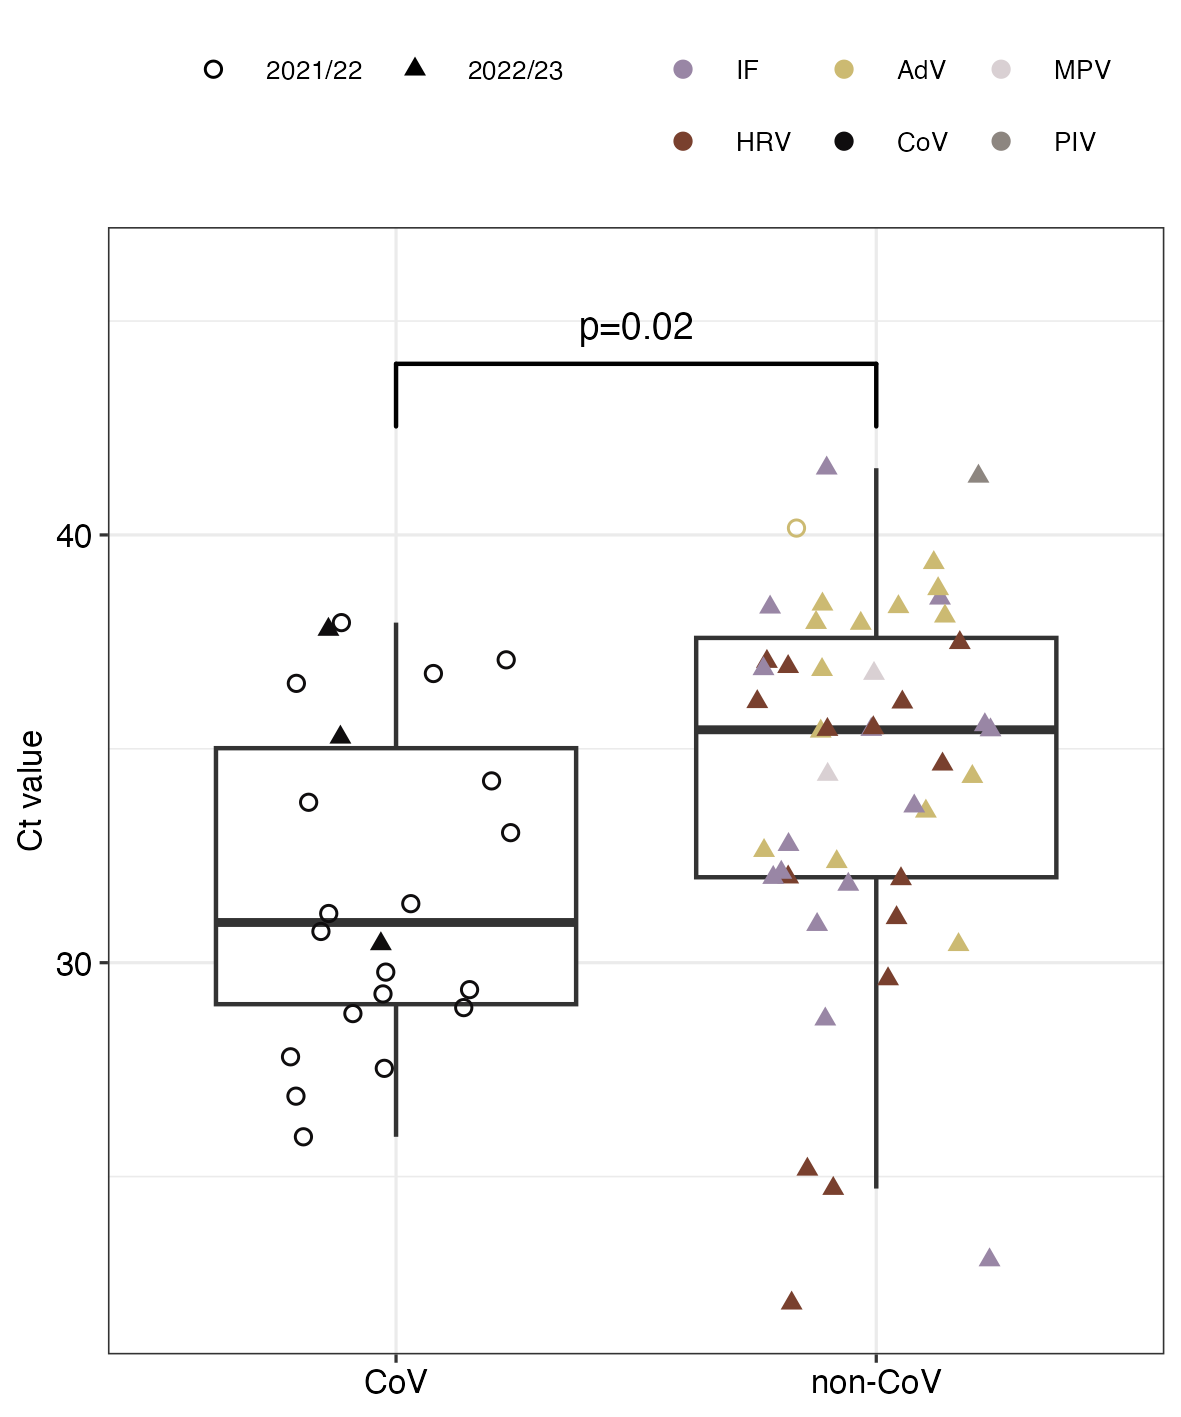
\includegraphics{results/comparison-viral-loads.png}
    \caption{Comparison of Ct values for positive saliva samples between SARS-CoV-2 (CoV) and non-SARS-CoV-2 (non-CoV) viruses. A statistical comparison was performed pooling the Ct values across the two study periods (winter 2021/22 and 2022/23), with the p-value (p) based on a numerical two-sided two sample t-test.}
    \label{fig:viral-loads}
\end{figure}

\clearpage

\section*{Model to estimate differences in airborne detection}\label{sec:model}

Our outcome is the binary variable $Y_{tcv}$ which is $1$ if any respiratory virus $v$ was detected in the air of classroom $c$ during study week $t$. We model this outcome with a Bayesian logistic regression model
\begin{align}
    \text{Bernoulli-Logit}(y|\mu) = \begin{cases}
        \text{logit}^{-1}(\mu) & \text{if }y=1\text{, and} \\
        1-\text{logit}^{-1}(\mu) & \text{if }y=0.
    \end{cases}
\end{align}
The parameter $\mu$ is related to the type of respiratory virus detected (SARS-CoV-2 vs non-SARS-CoV-2) and takes into account differences in the study setting (see \Cref{tab:comp_study}) as follows
\begin{align}
    \mu_{tcv} = \log(\text{offset}_c) + \alpha + \beta_1\,\cdot\text{saliva}_{tcv} + \beta_2\,\cdot\text{CoV}_{tcv} + \beta_3\,\cdot\text{mask}_{tc} + \beta_4\,\cdot\text{aircl}_{tc} + \beta_5\,\cdot\text{CO}_{2,tc}.
\end{align}
Since one classroom in 2022 was shared by two classes, we set the \textbf{offset} of this classroom to 2 (double odds for airborne detection in this classroom). Conversely, since one classroom in 2023 only had one instead of two sampling devices in place, we set the \textbf{offset} of this classroom to 0.5 (half odds for airborne detection in this classroom). Other classrooms have an offset of 1. The binary variable \textbf{saliva} indicates if there was a positive saliva sample in the same week, with $\beta_1$ estimating whether airborne detection was more frequent if the same virus was already detected in saliva. The binary variable \textbf{CoV} indicates if the detected virus was SARS-CoV-2, thus our parameter of interest $\beta_2$ is estimating whether airborne detection of any SARS-CoV-2 is more likely than non-SARS-CoV-2 viruses. The binary variables \textbf{masks} and \textbf{aircl} indicate if compulsory face mask wearing was mandated or portable air cleaners were installed in the classroom, respectively, with $\beta_3$ and $\beta_4$ estimating the change in the probability of airborne detection due to the intervention. The continuous variable \textbf{CO}$_2$ is the weekly average of the maximum daily CO$_2$ levels per classroom, with $\beta_5$ estimating the impact of CO$_2$ levels (a proxy for classroom ventilation) on the probability of airborne detection.

Considering the relatively small sample size and prior knowledge, we model the effects of the aforementioned variables with a mix of  non-informative and informative priors. The intercept is modeled with a non-informative prior
\begin{align}
    \alpha \sim \text{Student}(\nu=5, \mu = 0, \sigma = 2.5) ~.
\end{align}
Since bioaerosols were more frequently detected in weeks with a positive saliva sample, we model $\beta_1$ with an informative prior
\begin{align}
    \beta_1 \sim \text{Normal}(\mu = 5/3, \sigma = s_y / s_{\text{saliva}}),
\end{align}
where 5 is the number of weeks with paired samples and 3 is the number of weeks with a positive bioaerosol but without a positive saliva sample. The prior's hyperparameter for the standard deviation is computed as the ratio of the standard deviation of the outcome $s_y$ and predictor $s_{\text{saliva}}$. \\
Our parameter of interest $\beta_2$ is modeled with a non-informative prior
\begin{align}
    \beta_2 \sim \text{Normal}(\mu = 0, \sigma = s_y / s_\text{CoV})~.
\end{align}
Since masks and air cleaners possibly reduce the odds of airborne detection, we used informative asymmetric Laplace priors for $\beta_3$ and $\beta_4$ as follows
\begin{align}
    \beta_3 &\sim \text{Asymmetric-Laplace}(\mu = -0.32, \sigma = 0.5\cdot s_y / s_{\text{masks}}, \tau = 0.75) \\
    \beta_4 &\sim \text{Asymmetric-Laplace}(\mu = -0.27, \sigma = 0.5\cdot s_y / s_{\text{aircl}}, \tau = 0.75),
\end{align}
which both place 90\% prior probability on negative intervention effects (decreasing the odds of airborne detection) and are skewed towards smaller effect sizes. \\
Similarly, we incorporate our prior belief that higher CO$_2$ levels possibly increase the odds of airborne detection with an informative asymmetric Laplace prior for $\beta_5$ as
\begin{align}
    \beta_3 &\sim \text{Asymmetric-Laplace}(\mu = 0.21, \sigma = 0.5\cdot s_y / s_{\text{masks}}, \tau = 0.25)~,
\end{align}
which places 90\% prior probability on positive effects (increasing the odds of airborne detection).

To summarize, we estimate the probability of airborne detection of SARS-CoV-2, adjusting for differences in the setup of the classrooms (offset), positive saliva sample in the same week (saliva), the effects of interventions (masks and aircl), and differences in ventilation conditions (CO$_2$). We use informative priors for the parameters of the adjustments to incorporate prior knowledge and because the sample size and between-years comparison would otherwise make it difficult to identify these parameters. 

\clearpage

\end{document}